\chapter{Fusing of the two measurement sources}\label{ch:fusing}

The position of the object is estimated with an Extended Kalman Filter (EKF), using a model of the system and the measurements from the UWB as well as from the vision tracker. A block diagram of this pipeline is shown in \autoref{fig:block}.

\begin{figure}[h]\centering
	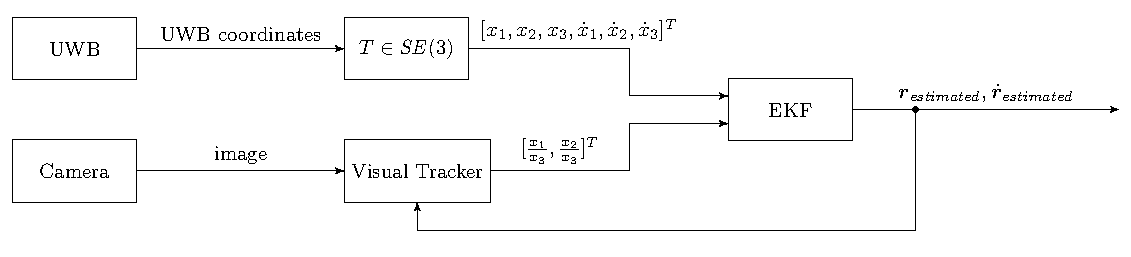
\includegraphics[width=1.0\textwidth]{figures/blockdiagram_setup}
	\caption{Block diagram of the EKF pipeline.}\label{fig:block}
\end{figure}

\section{Extended Kalman Filter (EKF)}

\subsection{System Model}
The state $\vec x = [\vec r, \dot{\vec{r}}]^T$ of our model consists of a position $\vec r \in \mathbb{R}^3$ and a velocity $\dot{\vec r} \in \mathbb{R}^3$.
The discrete process model with timestep $\Delta T$ is given by
\begin{equation}
	\vec x(k) = \vec q_{k-1}(\vec x(k-1), \vec v(k-1))
\end{equation}
with
\begin{equation}
  q_{k-1}(\vec x(k-1), \vec v(k-1)) = \textbf{B} \vec x(k-1) + \vec v(k-1)
\end{equation}
where 
\begin{align}
	\textbf{B} =
	\begin{pmatrix}
		\textbf{I}_3 & \Delta \textbf{T}\\
		\textbf{0} & \textbf{I}_3
	\end{pmatrix}
\end{align} 

and
\begin{equation}
	\vec v(k-1) \sim \mathcal{N}(\vec 0, \textbf{Q})
\end{equation}
where
\begin{align}
	\textbf{Q} =
	\begin{pmatrix}
		\textbf{I}_3 & \textbf{0}\\
		\textbf{0} & \textbf{q}_v
	\end{pmatrix}
\end{align}
and $\textbf{q}_v \in \mathbb{R}^{3\times3}$ is the velocity covariance of the process noise.

There are two possible measurements. The first measurement is a direct measurement of the state $\vec x$ from ultra-wideband (UWB) multilateration:
\begin{equation}
	\vec z_1(k) = \vec h_{k,1}(\vec x(k), \vec w_1(k))
\end{equation}
with
\begin{equation}
  \vec h_{k,1}(x(k), w_1(k)) = \textbf{H}_1 \vec x(k) + \vec w_1(k)
\end{equation}
where
$$\textbf{H}_1 = \textbf{I}_6$$
and
$$\vec \omega_1(k) \sim \mathcal{N}(\vec 0, \textbf{R}_1)$$
where $\textbf{R}_1 \in \mathbb{R}^{6\times6}$ is the covariance of the UWB measurement.
The second measurement is a projection of the position $\vec r$ as seen by a camera:
\begin{equation}
	\vec z_2(k) = \vec h_{k,2}(\vec x(k), \vec w_2(k))
\end{equation}
with
\begin{equation}
  \vec h_{k,2}(\vec x(k), \vec w_2(k)) = \textbf{H}_2(\vec x(k)) + \vec w_2(k)
\end{equation}
where
\begin{equation}
	\textbf{H}_2(\vec x) = [\frac{x_1}{x_3}, \frac{x_2}{x_3}]^T \in \mathbb{R}^2\\
\end{equation}
and
\begin{equation}
  \vec \omega_2(k) \sim \mathcal{N}(\vec 0, \textbf{R}_2)
\end{equation}

where $\textbf{R}_2 \in \mathbb{R}^{2\times2}$ is the covariance of the camera measurement.

\subsection{The Extended Kalman Filter steps}
There are two steps which have to be performed in an iterative fashion when running the Extended Kalman Filter (EKF).

\subsubsection{Step 1: Prior update/Prediction step}
In the first step, a prediction for the mean of the states $\hat{\vec x}_p(k)$ and the co-variance matrix $\textbf{P}_p(k)$ is calculated from the linearized system model.
\begin{align}
  \hat{\vec x}_p(k) &=  q_{k-1}(\hat{\vec x}_m(k-1), 0) = \textbf{B} \hat{\vec x}_m(k-1)\\
	\textbf{P}_p(k) &= {\textbf{A}}(k-1) \textbf{P}_m(k-1) {\textbf{A}}^T(k-1) + \textbf{L}(k-1) \textbf{Q} \textbf{L}^T(k-1) \label{eq:ekf_s1}
\end{align}
where
\begin{align}
  \textbf{A}(k-1) & = \frac{\partial q_{k-1}(\hat{\vec x}_m(k-1), 0)}{\partial \vec x}\\
  & =  \frac{\partial}{\partial \vec x} \big(\textbf{B} \vec x(k-1) + \vec v(k-1)\big)\\
	& = \textbf{B}(k-1)\\
  \textbf{L}(k-1) & = \frac{\partial q_{k-1}(\hat{\vec x}_m(k-1), 0)}{\partial \vec v}\\
  & = \frac{\partial}{\partial \vec v} \big( \textbf{B} \vec x(k-1) + \vec v(k-1)\big)\\
	& = \textbf{I}_6
\end{align}
and with the initial values $\hat{\vec x}_m(0) = x_0$ and $\textbf{P}_m(0) = \textbf{0}$.
Therefore equation \ref{eq:ekf_s1} becomes
$$\textbf{P}_p(k) = \textbf{B}(k-1)\textbf{P}_m(k-1)\textbf{B}^{T}(k-1) + \textbf{Q}$$

\subsubsection{Step 2: A posteriori update/Measurement update step}
In the second step, the information gained from the measurements are used to perform an a posteriori update, resulting in a updated mean of the states $\hat{\vec x}_m(k)$ and an updated co-variance matrix $\textbf{P}_m(k)$.
\begin{align}
	\textbf{K}(k) = \textbf{P}_p(k) \textbf{H}^T(k) \Big( \textbf{H}(k) \textbf{P}_p(k) \textbf{H}^T(k) + \textbf{M}(k) \textbf{R}(k) \textbf{M}^T(k)\Big)^{-1} \label{eq:ekf_s2}\\
	\hat{\vec x}_m(k) = \hat{\vec x}_p(k) + \textbf{K}(k) \Big( \vec z(k) - \begin{bmatrix}
	\vec h_{k,1}(\hat{\vec x}_p(k), 0)\\
	\vec h_{k,2}(\hat{\vec x}_p(k), 0))
	\end{bmatrix} \Big)\\
	\textbf{P}_m(k) = \big( \textbf{I} - \textbf{K}(k)\textbf{H}(k)\big) \textbf{P}_p(k)
\end{align}
where
\begin{align}
  \textbf{H}(k) &= \begin{bmatrix}
    \frac{\partial h_k(\hat{\vec x}_p(k), 0)}{\partial \vec x}
  \end{bmatrix}\\
  &= \begin{bmatrix}
		\frac{\partial}{\partial \vec x} \big( \textbf{H}_1 \hat{\vec x}(k) + \vec \omega_1(k) \big)\\
		\frac{\partial}{\partial \vec x} \big( \textbf{H}_2(\hat{\vec x}(k)) + \vec \omega_2(k) \big)
	\end{bmatrix}\\
	&= \begin{bmatrix}
		\textbf{I}_6\\
		\frac{1}{\hat{x}_3} & 0 & -\frac{\hat{x}_1}{\hat{x}^2_3} & 0 & 0 & 0\\
		0 & \frac{1}{\hat{x}_3} & -\frac{\hat{x}_2}{\hat{x}^2_3} & 0 & 0 & 0
	\end{bmatrix}\\
  \textbf{M}(k) & = \begin{bmatrix}
    \frac{\partial h_k(\hat{\vec x}_p(k), 0)}{\partial \vec w}
  \end{bmatrix}\\
  &= \begin{bmatrix}
		\frac{\partial}{\partial \vec \omega} \big( \textbf{H}_1 \hat{\vec x}(k) + \vec \omega_1(k) \big)\\
		\frac{\partial}{\partial \vec \omega} \big( \textbf{H}_2(\hat{\vec x}(k)) + \vec \omega_2(k) \big)
	\end{bmatrix}\\
	&= \textbf{I}_8
\end{align}
Therefore equation \ref{eq:ekf_s2} becomes
$$\textbf{K}(k) = \textbf{P}_p(k) \textbf{H}^T(k) \Big( \textbf{H}(k) \textbf{P}_p(k) \textbf{H}^T(k) + \begin{bmatrix}
	\textbf{R}_1 & \textbf{0}\\
	\textbf{0} &\textbf{R}_2
\end{bmatrix} \Big)^{-1}$$

\subsection{Implementation}
The implementation of the EKF was done in a Python script within the ROS environment. For more details please see \autoref{}.

\begin{figure}[ht!]\centering
	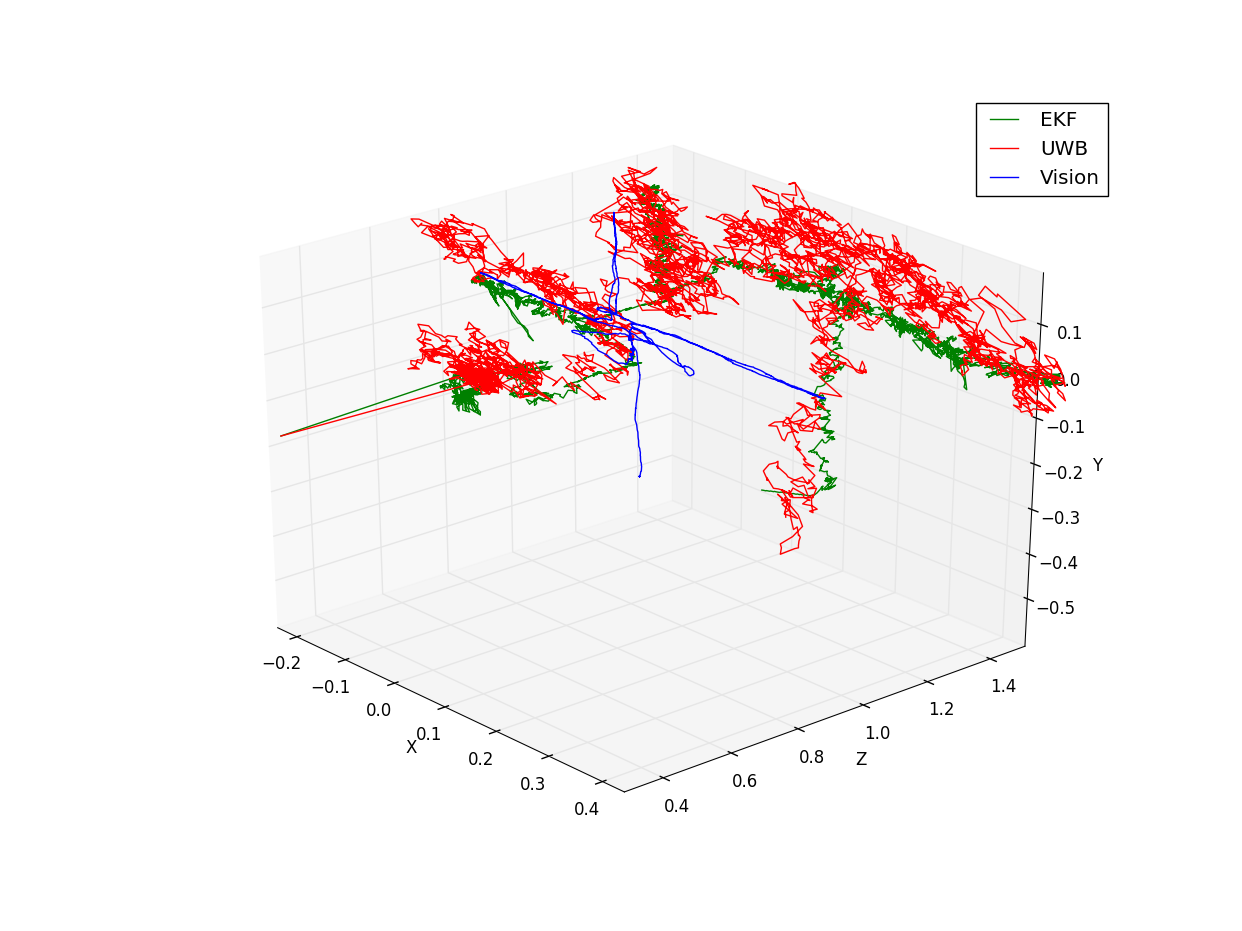
\includegraphics[width=1.0\textwidth]{figures/state_track}
	\caption{3D pot of the measured point by the UWB (red), the measured point by the vision tracker (blue) and the fused positions (green)}\label{fig:statetrack}
\end{figure}
